\section{Banken}
Banken erwirtschaften ihren Gewinn durch: Kreditvergabe mit geliehenem Geld (Zinsdifferenzgeschäft), Kommissionsgeschäft (Vermögensverwaltung, Investmentbanking), Eigenhandel.
\begin{itemize}
	\item Finanzierung von Unternehmen: entweder direkte Finanzierung durch Aktien und Obligationen oder durch indirekte Finanzierung durch die Banken. Bei Beiden sind die Haushalte der Ursprung.
	\item Banken als Finanzintermediäre (Zwischenliegende)
	Sie vermitteln das Kapital zwischen den Anlegern (den Haushalten) und den Kreditnehmern. Sie lösen dabei drei Probleme: 
	\subitem 1. Transformation von Fristen
	\subitem 2. Breitstellen von Informationen (an Kreditgeber und Nehmer)
	\subitem 3. Verteilung des Risikos bei Kreditausfall
	\item Die Banken sind immer stark verschuldet 
\end{itemize}
\begin{figure*}[h]
	\centering
	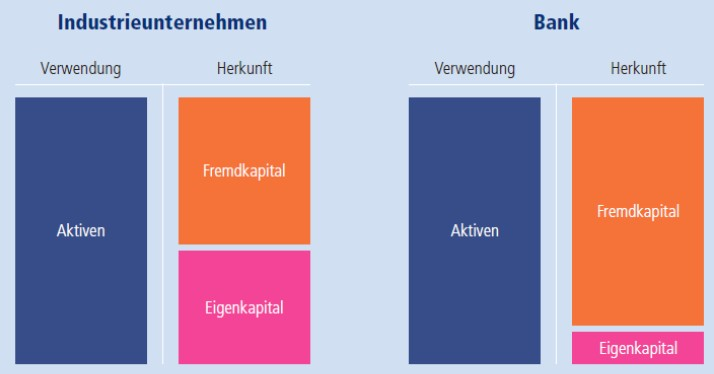
\includegraphics[width=0.7\linewidth]{images/banken.jpg}
\end{figure*}
\subsection{Risiken des Bankgeschäfts}
\begin{itemize}
	\item \textbf{Liquiditätsrisiko (Passivseite):} Falls die Kreditgeber (Haushalte) massenweise ihr Geld zurückfordern Bank-Run.
	\item \textbf{Solvenzrisiko (Aktivseite):}  Wenn die Bank auf der Aktivseite (verliehene Kredite) Verluste erleidet.Zum Beispiel bei Kreditausfällen oder Werteminderung der Wertpapieren. Diese Verluste müssen mit dem Eigenkapital gedeckt werden können. 
\end{itemize}
\subsection{Bankenregulierung}
Die Banken gehören zu den stärksten regulierten Branchen. Als Schutz für die Kunden und für die Stabilität des Finanzsystems.\\
\begin{minipage}{13cm}
	\begin{itemize}
		\item \textbf{Mikroprudentielle Regulierung (Stabilität einzelner Banken): } Aufgabe der FINMA-> kontrolliert Eigenkapital und Liquiditätsaustattung.
		\item \textbf{Makroprudentielle Regulierung (Stabilität des gesamten Bankensystems): }Aufgabe der SNB, sie setzt dabei auf Beobachtung und Entwicklung der Finanzmärkte (Prävention), wirkt bei den rechtlichen Rahmenbedingung mit und bietet eine Kurzfristige Vorsorge im Krisenfall.
	\end{itemize}
\end{minipage}
\begin{minipage}{6cm}
	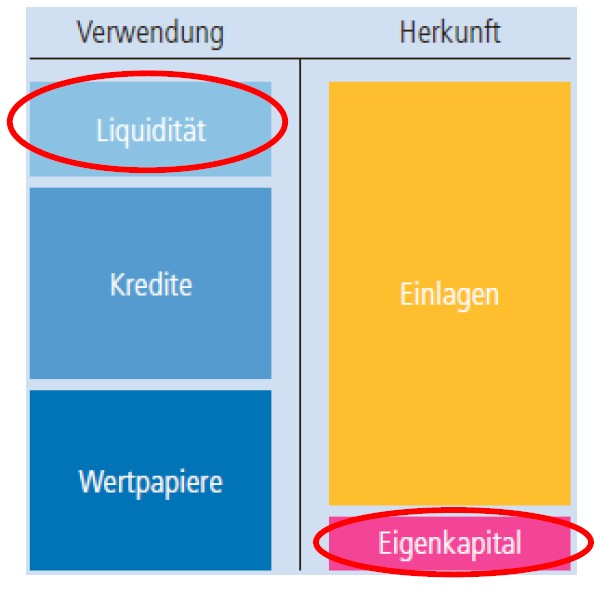
\includegraphics[width=6cm]{images/banken2.jpg}
\end{minipage}
\clearpage
\pagebreak
\subsubsection{Vorschriften}
\begin{itemize}
	\item Eigenkapitalvorschriften (Passivseite)
	\subitem Basel II (8\%) und Basel III (13\%)
	\item Liquiditätsvorschriften
	\subitem Obligatorische Einlageversicherung. Dies verhindert Bank-Runs, da der Kunde weiss, dass er sein Geld (bis zu einer definierten Obergrenze) trotz Liquiditätsproblemen der Bank zurück erhält.
	\subitem Liquiditätsvorgaben: Die Bank muss einen bestimmten Prozentsatz der Aktiven als flüssige Mittel
	halten. Dies ist für die Banken teuer (sie hat keine Erträge aus diesen Mitteln). Deshalb versuchen sich die Banken vor allem auf dem Geldmarkt bei anderen Banken zu finanzieren, da dieses Kapital in der Regel günstiger ist als das zur Verfügung gestellte Kapital der Haushalte.
	\item Makroprudentielle Vorschriften zur Konkursabwicklung
\end{itemize}
\subsubsection{Too Big to Fail}
Die gegenseitige kurzfristige Finanzierung von Banken in Form des Interbanken-Geschäfts (zwecks Liquiditätssicherung, aber teilweise auch für den Eigenhandel) führt zu einer starken Verflechtung des Bankensektors. Kommt es zu einem Bank-Run bei einer grossen Bank, können auch andere kreditgebende Banken unter Druck geraten.In einem solchen Fall müssen Zentralbanken bzw. Regierungen die insolventen Banken retten. Ein Scheitern dieser Banken würde unabsehbare Folgen für die Volkswirtschaft mit sich ziehen. Dies schafft eine unhaltbare Situation: die Banken werden ihre Risiken maximieren. Die Gewinne werden damit privatisiert, während die Allgemeinheit für die allfällige Verluste aufkommen muss (entspricht faktisch einer Staatsgarantie).\\
\textbf{Lösung dazu}\\
\begin{itemize}
	\item 1. Insolvenzverhinderung durch höhere Eigenkapitalforderung
	\item 2. Verfahren zur Konkursabwicklung beschrieben in Form eines living will (funktionsfähige Geschäftsbereiche abspalten)
\end{itemize}

